\section{Development Environment}
%The basic purpose for this section is to give a developer all of the necessary 
%information to setup their development environment to run, test, and/or develop. 
Microsoft's Development environment was chosen for this project. This environment
was chosen for the following reasons:

\begin{itemize}
    \item Azure allows for simple cloud hosting and database integration.

    \item Student Licenses give certain paid feature of Azure for free.
    
    \item Access to Visual Studio is free through student accounts.

    \item Developers were comfortable working with the ASP.NET MVC framework.

    \item Microsoft is the owner of the targeted device, The HoloLens.

    \item Unity is used for HoloLens app development which has a C\# backing making it necessary to us Microsoft environment.

    \item Androids study was chosen because it is the default for Android application development.

\end{itemize}

\section{Development IDE and Tools}
%Describe which IDE and provide links to installs and/or reference material. 
Many IDE and tools are used to create this project. Below is a list of those
tools with descriptions:

\begin{itemize}

    \item Website IDE and Tools
    \begin{itemize}
        \item Visual Studio 2017 Enterprise - Microsoft's code editor. Allows for easy Azure and database
        integration. Also allows for easy installation of the Unity Development Tools.
        \item ASP.NET MVC - Microsoft's framework for creating websites.
        \item Azure Cloud Tools - Tools that allow for easy integration with Azure, able to install in Visual Studio Installer
    \end{itemize}

    \item File Conversion and Tools
    \begin{itemize}
        \item Autodesk's FBX SDK is required to export FBX files.  It must be installed in a folder located in the project directory named "FBX SDK".  The download can be found at: 
        \url{http://usa.autodesk.com/adsk/servlet/pc/item?siteID=123112&id=26416244}.
        The Windows VS2015 version must be installed.

        \item Open Asset Import Library supports a wide variety of import and export file types.  The download can be found at: \url{http://assimp.org/main_downloads.html}.  Version 3.1.1 is what was used in the project.         
    \end{itemize}

    \item HoloLens Development Tools
    \begin{itemize}
        \item Visual Studio 2017 - Community version is okay. Make sure to select Windows Universal Development and Unity Game Development options enabled.

        \item Unity Personal - Free version of Unity editor used for creating HoloLens app

        \item HoloToolkit - Free Set of tools you can download from an open source GitHub Project

        \item HoloLens Emulator - Free Microsoft Emulator. Warning! Must enable Hyper-V, which disrupts other visualization software.

    \end{itemize}

    \item Android Development Tools
    \begin{itemize}
        \item Android Studio
        \item ARCore (from the Google Play Store)
    \end{itemize}
\end{itemize}


\section{Source  Control}
\subsection{Source Control Tool}
GitHub was used to provide source control and a private repository. This tool was chosen over others available as it is unanimously familiar to all developers. 

\subsection{Source Control Architecture}
The repository was created with the following three branches: Master, Develop and Release. 
Develop is used for work in progress. After features have been verified through thorough testing, they are merged into the Release branch for beta usage. Once verified in Release, features are merged into the Master branch is reserved for the final deliverable. 


\subsection{Source Control Etiquette}
The following steps represent the code flow process: 

\begin{enumerate}
\item Pull latest code from the develop branch
\item Implement feature
\item Push to Develop and assign other developer for QA
\item Once properly tested, merge feature into Release branch
\item Once feature verified in Release, merge feature into Master
\end{enumerate}

\subsection{Developer Contributions}
Figure \ref{Contributions} shows a snapshot of repository activity and developer contributions:

\begin{figure}[H]
	\centering
	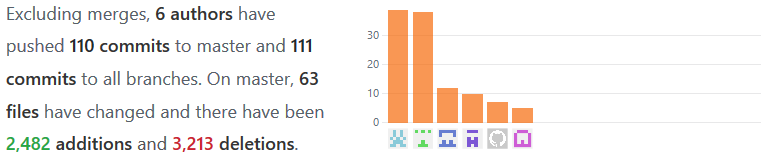
\includegraphics[width=\textwidth]{Contributions.png}
	\caption{Developer Contributions} 
	\label{Contributions}	
\end{figure}



\section{Dependencies}
%Describe all dependencies associated with developing the system. 
\paragraph{Website}
\begin{itemize}
    \item Visual Studio 2017 Enterprise - Microsoft's code editor. Allows for easy Azure and database
    integration. Also allows for easy installation of the Unity Development Tools.
    \item ASP.NET MVC - Microsoft's framework for creating websites.
    \item Azure Cloud Tools - Tools that allow for easy integration with Azure, able to install in Visual Studio Installer
\end{itemize}

\paragraph{File Conversion}
\begin{itemize}
    \item Autodesk's FBX SDK is required to export FBX files.  It must be installed in a folder located in the project directory named \"FBX SDK\".  The download can be found at: 
    \url{http://usa.autodesk.com/adsk/servlet/pc/item?siteID=123112&id=26416244}.
    The Windows VS2015 version must be installed.

    \item Open Asset Import Library supports a wide variety of import and export file types.  The download can be found at: \url{http://assimp.org/main_downloads.html}.  Version 3.1.1 is what was used in the project.         
\end{itemize}

\paragraph{HoloLens App}
\begin{itemize}
    \item Visual Studio 2017 - Community version works.  Make sure to select Windows Universal Development and Unity Game Development options enabled.
    
    \item Unity Personal - Free version of Unity editor used for creating HoloLens app

    \item HoloToolkit - Free Set of tools you can download from an open source GitHub Project
\end{itemize}

\paragraph{Android App}
\begin{itemize}
    \item Android Studio - IDE for Android development
    \item ARCore - Support for AR on Android devices (off of the Google Play Store)
    \begin{itemize}
        \item Only works on specific devices (as of 4/26/2018)
        \item Use OpenGL to draw models, ARCore only performs tracking/world mapping
    \end{itemize}
    \item OBJ Parser
    \begin{itemize}
        \item Used by the example AR Core application to draw the model
        \item Parses the OBJ files
        % \item \url{https://github.com/JohnLXiang/arcore-sandbox}
    \end{itemize}
    \item QR Code Reader - included in Android project dependencies
    \item Volley - Google library for network communications between app and website
    \item Room - Google library that provides an abstraction layer over SQLite for storing file listings in the phone's database.
\end{itemize}

\section{Build  Environment}
Azure is used to build and deploy the website. Once the tools are downloaded and an Azure account is created, 
all that is needed is to right-click on the ASP.NET MVC project and select publish. The website is then hosted on Azure and
can be accessed by all.
Android Studio is used to build the mobile app. After setting up the environment for normal development, Android Studio builds the app for the desired device (connected for debugging) or it can be specified to build a release APK for distribution. 

\section{Development Machine Setup}

Pull the git repository with the Website, File Conversion, and Android code located at: \url{https://github.com/SavoySchuler/ARFE}

% If warranted, provide a list of steps and details associated with setting up a 
% machine for use by a developer. 

The following are the requirements for a development machine:
\begin{itemize}
    \item Windows 10
    \item Visual Studio 2017 Enterprise with ASP.NET MVC, Azure and Unity tools
    \item Unity Personal
    \item HoloToolkit-Unity Set of tools for Hololens development with unity. Free for use. Download from the GitHub page.
    \item Android Studio for Android app development
\end{itemize}

\paragraph{File Conversion}

There are two libraries that need to be installed: Assimp and FBX SDK.

\subparagraph{FBX SDK}

\begin{enumerate}
    \item Go to the following link and install the FBX SDK.
    \begin{itemize}
        \item \url{http://usa.autodesk.com/adsk/servlet/pc/item?siteID=123112&id=26416244}
        \item Use the installer under: Windows / FBX SDK 2018.0 VS2015
    \end{itemize}

    \item Copy the FBX SDK folder to the directory with the source code (the deepest FileConverion folder)
    \begin{itemize}
        \item At the location of the installation, the file structure should be: Autodesk/FBX/FBX SDK/
        \item Copy the FBX SDK folder to the source code directory.
    \end{itemize}
\end{enumerate}

\subparagraph{Assimp}

\begin{enumerate}
    \item Go to the following link and install the Assimp software.
    \begin{itemize}
        \item \url{http://assimp.org/main_downloads.html}
        \item Version 3.1.1 is what was used during development.
    \end{itemize}

    \item From the installation location, copy the \"Assimp\" folder into the deeper FileConversion directory.
    \begin{itemize}
        \item Paste the folder into the same folder as the source code of the File Conversion.
    \end{itemize}

    \item Copy FileConverion/Assimp/bin/x86/assimp-vc140-mt.dll to the same directory as the source code.
\end{enumerate}

\paragraph{Android Development}

\subparagraph{PC Setup}
\begin{enumerate}
    \item Install Android Studio
    \begin{itemize}
        \item \url{https://developer.android.com/studio/index.html}
    \end{itemize}
    \item Dependencies are automatically included with the Android Studio project.
    \item Android Studio requires specific build tools to be installed for the target device's android version. Follow prompts when building the app and Android Studio installs necessary components for you.

\end{enumerate}

\subparagraph{Mobile Device Setup}
\begin{enumerate}
    \item Install Android Studio
    \item Enable developer mode on the Android device
    \begin{itemize}
        \item \url{https://developer.android.com/studio/debug/dev-options.html}
        \item Make sure to enable remote debugging from the developer settings on the device
        \item On the device, make sure to set the computer as a trusted device for debugging when prompted.
        \item Extra device drivers may need to be installed on the development computer
    \end{itemize}

    \item Install ARCore from the Play Store
\end{enumerate}